\documentclass[tikz,border=6pt]{standalone}

% общий стиль (подключается через TEXINPUTS)
% tikz-style.tex (общий стиль для всех TikZ-картинок)
\RequirePackage[T1,T2A]{fontenc}
\RequirePackage[utf8]{inputenc}

% Palatino-подобный шрифт (как в MathJax часто воспринимается «более вытянутым»)
\RequirePackage{txfonts}
% txfonts даёт предупреждение по кириллице (T2A/txr не определён).
% Оставляем txfonts для математики, а текстовый шрифт возвращаем на Computer Modern,
% чтобы не искать T2A/txr и убрать предупреждения.
\renewcommand{\rmdefault}{cmr}
\renewcommand{\sfdefault}{cmss}
\renewcommand{\ttdefault}{cmtt}

\RequirePackage{tikz}
\RequirePackage{xcolor}
\usetikzlibrary{calc}

% цвета
\definecolor{lightgreen}{RGB}{214,234,214}
\definecolor{darkgreen}{HTML}{0B7A0B}
\definecolor{darkred}{HTML}{DF0000}

\definecolor{midgreen}{HTML}{2E9B2E}
\definecolor{palegreen}{RGB}{235,246,235}
\definecolor{olivegreen}{HTML}{3E6B2F}

\definecolor{lightred}{RGB}{255,220,220}
\definecolor{midred}{HTML}{E04545}
\definecolor{darkred2}{HTML}{A80000}

\definecolor{lightblue}{RGB}{220,232,255}
\definecolor{midblue}{HTML}{2E5BD6}
\definecolor{darkblue}{HTML}{0B2E8A}

\definecolor{lightgray}{RGB}{240,240,240}
\definecolor{midgray}{RGB}{170,170,170}
\definecolor{darkgray}{RGB}{80,80,80}

\definecolor{vtxfill}{RGB}{86,193,255}
\definecolor{vennfill}{RGB}{220,232,255}


% единый набор стилей TikZ
\tikzset{
    lab/.style={
        font=\fontsize{24}{32}\selectfont
    }
}


\begin{document}
  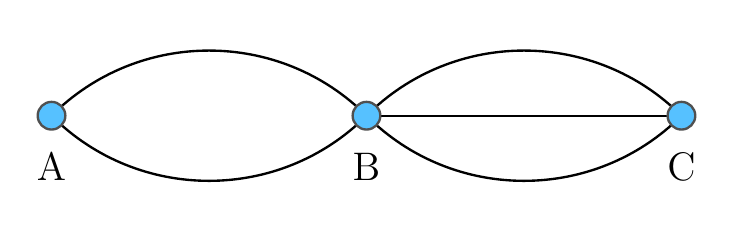
\begin{tikzpicture}[x=1cm,y=1cm, line cap=round, line join=round]

    \tikzset{
      main/.style={draw=black, line width=0.85pt},
      vtx/.style={circle, draw=darkgray, fill=vtxfill, line width=0.85pt, minimum size=10pt, inner sep=0pt},
      vlab/.style={font=\Large},
    }

    \coordinate (A) at (0,0);
    \coordinate (B) at (4,0);
    \coordinate (C) at (8,0);

% parallel edges A--B
    \draw[main] (A) to[out=45,in=135] (B);
    \draw[main] (A) to[out=-45,in=-135] (B);

% parallel edges B--C (upper + lower + straight)
    \draw[main] (B) to[out=45,in=135] (C);
    \draw[main] (B) to[out=-45,in=-135] (C);
    \draw[main] (B) -- (C);

% vertices
    \node[vtx] at (A) {};
    \node[vtx] at (B) {};
    \node[vtx] at (C) {};

% vertex labels
    \node[vlab, anchor=north] at ($(A)+(0,-0.35)$) {A};
    \node[vlab, anchor=north] at ($(B)+(0,-0.35)$) {B};
    \node[vlab, anchor=north] at ($(C)+(0,-0.35)$) {C};

  \end{tikzpicture}
\end{document}